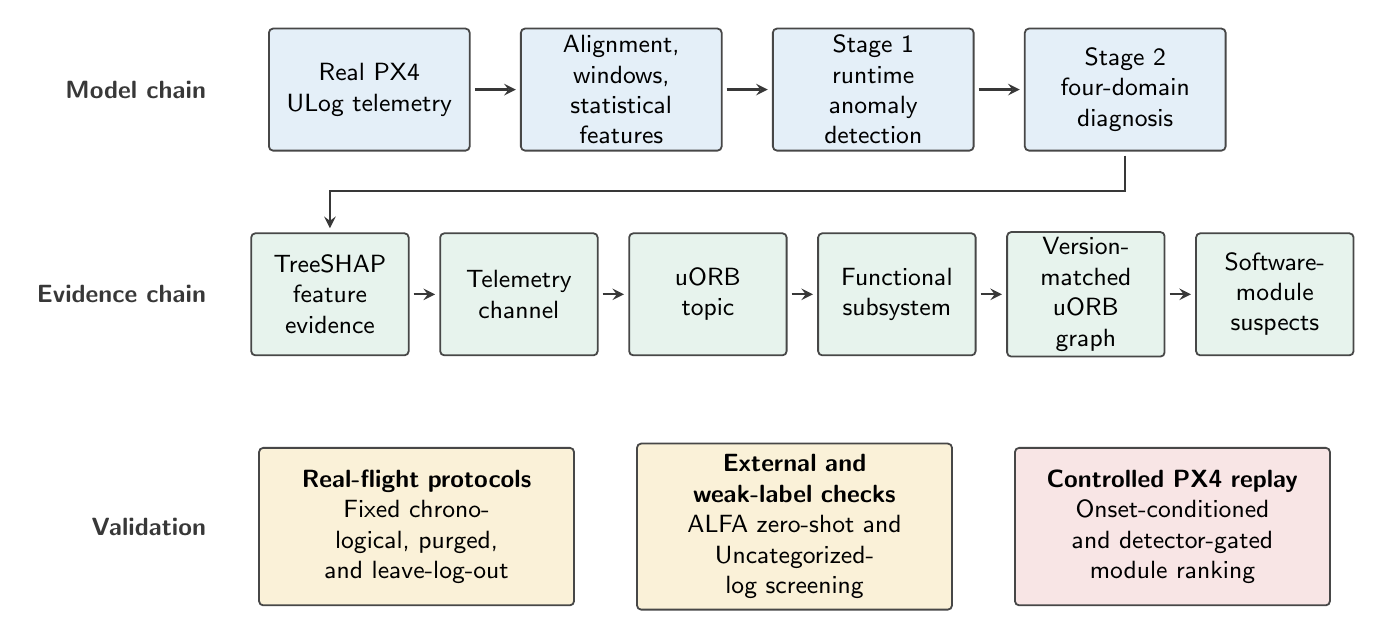
\begin{tikzpicture}[
    font=\sffamily\small,
    block/.style={draw=black!72, rounded corners=1.5pt, line width=0.65pt, align=center, minimum width=2.55cm, minimum height=1.55cm, text width=2.15cm, inner sep=2pt},
    evidence/.style={draw=black!72, rounded corners=1.5pt, line width=0.65pt, align=center, minimum width=2.00cm, minimum height=1.55cm, text width=1.70cm, inner sep=2pt},
    validation/.style={draw=black!72, rounded corners=1.5pt, line width=0.65pt, align=center, minimum width=4.00cm, minimum height=2.00cm, text width=3.55cm, inner sep=4pt},
    flow/.style={->, draw=black!78, line width=0.85pt, >=stealth, shorten <=1.5pt, shorten >=1.5pt},
    rowlabel/.style={anchor=east, font=\sffamily\bfseries\small, text=black!78}
]
\definecolor{modelblue}{RGB}{228,239,248}
\definecolor{evidencegreen}{RGB}{231,243,237}
\definecolor{validationgold}{RGB}{250,241,216}
\definecolor{boundaryred}{RGB}{248,229,229}

\node[rowlabel] at (-0.15,4.70) {Model chain};
\node[block, fill=modelblue] (ulog) at (1.80,4.70) {Real PX4\\ULog telemetry};
\node[block, fill=modelblue] (features) at (5.00,4.70) {Alignment, windows,\\statistical features};
\node[block, fill=modelblue] (stage1) at (8.20,4.70) {Stage 1\\runtime anomaly\\detection};
\node[block, fill=modelblue] (stage2) at (11.40,4.70) {Stage 2\\four-domain\\diagnosis};
\draw[flow] (ulog) -- (features);
\draw[flow] (features) -- (stage1);
\draw[flow] (stage1) -- (stage2);

\node[rowlabel] at (-0.15,2.10) {Evidence chain};
\node[evidence, fill=evidencegreen] (shap) at (1.30,2.10) {TreeSHAP\\feature\\evidence};
\node[evidence, fill=evidencegreen] (channel) at (3.70,2.10) {Telemetry\\channel};
\node[evidence, fill=evidencegreen] (topic) at (6.10,2.10) {uORB\\topic};
\node[evidence, fill=evidencegreen] (subsystem) at (8.50,2.10) {Functional\\subsystem};
\node[evidence, fill=evidencegreen] (graph) at (10.90,2.10) {Version-matched\\uORB graph};
\node[evidence, fill=evidencegreen] (suspects) at (13.30,2.10) {Software-module\\suspects};
\draw[flow] (shap) -- (channel);
\draw[flow] (channel) -- (topic);
\draw[flow] (topic) -- (subsystem);
\draw[flow] (subsystem) -- (graph);
\draw[flow] (graph) -- (suspects);
\draw[flow] (stage2.south) -- ++(0,-0.50) -| (shap.north);

\node[rowlabel] at (-0.15,-0.85) {Validation};
\node[validation, fill=validationgold] (internal) at (2.40,-0.85) {\textbf{Real-flight protocols}\\Fixed chronological, purged,\\and leave-log-out};
\node[validation, fill=validationgold] (external) at (7.20,-0.85) {\textbf{External and weak-label checks}\\ALFA zero-shot and\\Uncategorized-log screening};
\node[validation, fill=boundaryred] (replay) at (12.00,-0.85) {\textbf{Controlled PX4 replay}\\Onset-conditioned and detector-gated\\module ranking};
\end{tikzpicture}
